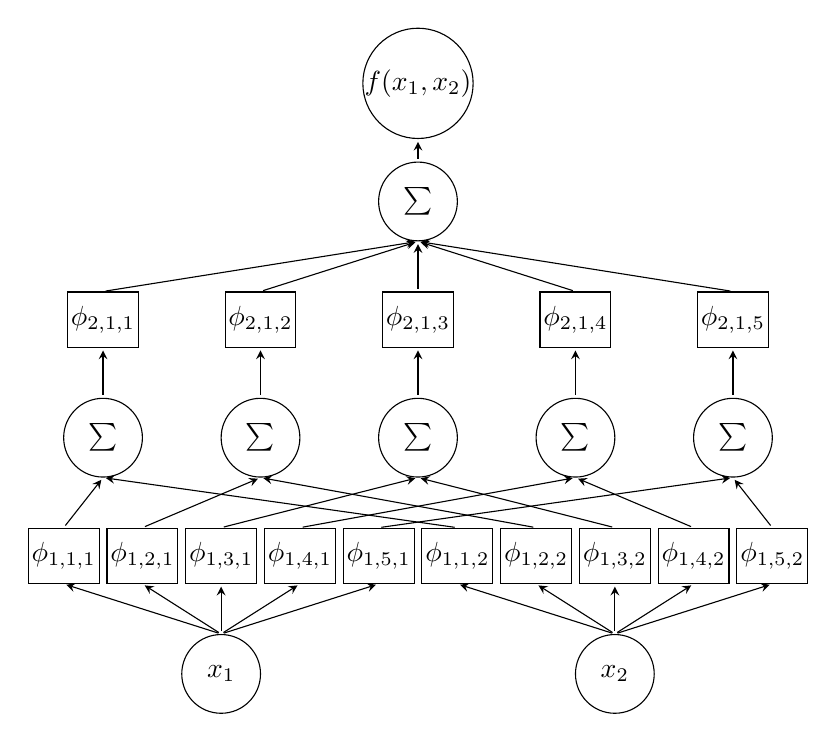
\begin{tikzpicture}[
	neuron/.style={circle, draw, minimum size=10mm, inner sep=0pt},
	box/.style={draw, rectangle, minimum width=9mm, minimum height=7mm, inner sep=1pt, fill=white},
	>=stealth
	]
	
	%-----------------------
	% Customizable heights
	%-----------------------
	\def\hin{0}      % Row 1: inputs
	\def\hphi{1.5}   % Row 2: phi_{i,j} squares
	\def\hsum{3}     % Row 3: per-column sums
	\def\hPhi{4.5}   % Row 4: Phi_j squares
	\def\hsumall{6}  % Row 5: global sum
	\def\hout{7.5}   % Row 6: output
	
	%-----------------------
	% Row 1: inputs
	%-----------------------
	\node[neuron] (X1) at (-2.5,\hin) {$x_1$};
	\node[neuron] (X2) at ( 2.5,\hin) {$x_2$};
	
	%-----------------------
	% Row 2: phi_{i,j} squares
	%-----------------------
	\node[box] (phi111) at (-4.5,\hphi) {$\phi_{1,1,1}$};
	\node[box] (phi121) at (-3.5,\hphi) {$\phi_{1,2,1}$};
	\node[box] (phi131) at (-2.5,\hphi) {$\phi_{1,3,1}$};
	\node[box] (phi141) at (-1.5,\hphi) {$\phi_{1,4,1}$};
	\node[box] (phi151) at (-0.5,\hphi) {$\phi_{1,5,1}$};
	
	\node[box] (phi112) at (0.5,\hphi) {$\phi_{1,1,2}$};
	\node[box] (phi122) at (1.5,\hphi) {$\phi_{1,2,2}$};
	\node[box] (phi132) at (2.5,\hphi) {$\phi_{1,3,2}$};
	\node[box] (phi142) at (3.5,\hphi) {$\phi_{1,4,2}$};
	\node[box] (phi152) at (4.5,\hphi) {$\phi_{1,5,2}$};
	
	%-----------------------
	% Row 3: per-column sums
	%-----------------------
	\node[neuron] (S-1) at (-4,\hsum) {$\textstyle\sum$};
	\node[neuron] (S-2) at (-2,\hsum) {$\textstyle\sum$};
	\node[neuron] (S-3) at ( 0,\hsum) {$\textstyle\sum$};
	\node[neuron] (S-4) at ( 2,\hsum) {$\textstyle\sum$};
	\node[neuron] (S-5) at ( 4,\hsum) {$\textstyle\sum$};
	
	%-----------------------
	% Row 4: Phi_j squares
	%-----------------------
	\node[box] (phi211) at (-4,\hPhi) {$\phi_{2,1,1}$};
	\node[box] (phi212) at (-2,\hPhi) {$\phi_{2,1,2}$};
	\node[box] (phi213) at ( 0,\hPhi) {$\phi_{2,1,3}$};
	\node[box] (phi214) at ( 2,\hPhi) {$\phi_{2,1,4}$};
	\node[box] (phi215) at ( 4,\hPhi) {$\phi_{2,1,5}$};
	
	%-----------------------
	% Row 5: global sum
	%-----------------------
	\node[neuron] (Sall) at (0,\hsumall) {$\textstyle\sum$};
	
	%-----------------------
	% Row 6: output
	%-----------------------
	\node[neuron] (F) at (0,\hout) {$f(x_1,x_2)$};
	
	%-----------------------
	% Connections (use top/bottom anchors)
	%-----------------------
	\tikzset{connect/.style={->,shorten >=1pt,shorten <=1pt}}
	
	% Inputs -> phi (into phi from below)
	\draw[connect] (X1.north) -- (phi111.south);
	\draw[connect] (X1.north) -- (phi121.south);
	\draw[connect] (X1.north) -- (phi131.south);
	\draw[connect] (X1.north) -- (phi141.south);
	\draw[connect] (X1.north) -- (phi151.south);
	
	\draw[connect] (X2.north) -- (phi112.south);
	\draw[connect] (X2.north) -- (phi122.south);
	\draw[connect] (X2.north) -- (phi132.south);
	\draw[connect] (X2.north) -- (phi142.south);
	\draw[connect] (X2.north) -- (phi152.south);
	
	% phi -> per-column sums (enter sums from below)
	\draw[connect] (phi111.north) -- (S-1.south);
	\draw[connect] (phi112.north) -- (S-1.south);
	\draw[connect] (phi121.north) -- (S-2.south);
	\draw[connect] (phi122.north) -- (S-2.south);
	\draw[connect] (phi131.north) -- (S-3.south);
	\draw[connect] (phi132.north) -- (S-3.south);
	\draw[connect] (phi141.north) -- (S-4.south);
	\draw[connect] (phi142.north) -- (S-4.south);
	\draw[connect] (phi151.north) -- (S-5.south);
	\draw[connect] (phi152.north) -- (S-5.south);
	
	% sums -> Phi (upwards)
	\draw[connect] (S-1.north) -- (phi211.south);
	\draw[connect] (S-2.north) -- (phi212.south);
	\draw[connect] (S-3.north) -- (phi213.south);
	\draw[connect] (S-4.north) -- (phi214.south);
	\draw[connect] (S-5.north) -- (phi215.south);
	
	% Phi -> global sum
	\draw[connect] (phi211.north) -- (Sall.south);
	\draw[connect] (phi212.north) -- (Sall.south);
	\draw[connect] (phi213.north) -- (Sall.south);
	\draw[connect] (phi214.north) -- (Sall.south);
	\draw[connect] (phi215.north) -- (Sall.south);
	
	% Global sum -> output
	\draw[connect] (Sall.north) -- (F.south);
	
\end{tikzpicture}